% THIS TEMPLATE IS A WORK IN PROGRESS
% Adapted from an original template by faculty at Reykjavik University, Iceland

\documentclass{scrartcl}

% Adapted from an original template by Hlyni Arnórssyni, Reykjavik University, Iceland
%
% ------------------------------ SETTINGS
\usepackage{geometry}

\geometry{
	paper=a4paper, % Paper size
	top=2.5cm, % Top margin
	bottom=2.5cm, % Bottom margin
	left=2.5cm, % Left margin
	right=2.4cm, % Right margin
	headheight=0.75cm, % Header height
	footskip=1.5cm, % Space from the bottom margin to the baseline of the footer
	headsep=0.75cm, % Space from the top margin to the baseline of the header
	%showframe, % Uncomment to show how the type block is set on the page
}

\usepackage{blindtext}
%-------------------------------- Character encoding ----------------------------
\usepackage[T1]{fontenc}
\usepackage[utf8]{inputenc}

%----------------------------- Mathematics packages from AMS ---------------

\usepackage{amsmath, amsfonts, amsthm, amssymb}
\usepackage{braket, nicefrac}

% ----------- International System of Units
\usepackage{siunitx}

%------------------------------ Lists / numbers -------------------------
\usepackage{enumitem, multicol}

%------------------------------- Figure insertions --------------
\usepackage{graphicx, float}  % Use option [H] to force the placement of a figure
\usepackage{keystroke}
\usepackage{pgfplots}\usepgfplotslibrary{units}\pgfplotsset{compat=1.16}

%------------------------------- Line Spacing --------------
\usepackage{setspace}

%------------------------------- Depth of the ToC --------------
\setcounter{tocdepth}{2}

%%%%%%%%%%%%%%%%%%%%%%%%%% Hyperlink References %%%%%%%%%%%%%%%%%%%%%%%%%%%
\usepackage{hyperref}

%--------------------% Storage Path for images %-----------------%
\graphicspath{{graphics/}{Graphics/}{./}}

%%%%%%%%%%%%%%%%%%%%%%%%%% Environments %%%%%%%%%%%%%%%%%%%%%%%%%%%
\renewenvironment{abstract}{
    \begin{center}
    \textbf{Abstract}
    \vspace{0.5cm}
    \par\itshape
    \begin{minipage}{0.8\linewidth}}{\end{minipage}
    \noindent\ignorespaces
    \end{center}
}

\newenvironment{keywords}{
    \begin{center}
    \textbf{Keywords}
    \vspace{0.5cm}
    \par
    \begin{minipage}{0.8\linewidth}}{\end{minipage}
    \noindent\ignorespaces
    \end{center}
}

\newenvironment{preface}{
    \begin{center}
    \textbf{Preface}
    \vspace{0.5cm}
    \par
    \begin{minipage}{0.8\linewidth}}{\end{minipage}
    \noindent\ignorespaces
    \end{center}
}

\newenvironment{acknowledgements}{
    \begin{center}
    \textbf{Acknowledgements}
    \vspace{0.5cm}
    \par
    \begin{minipage}{0.8\linewidth}}{\end{minipage}
    \noindent\ignorespaces
    \end{center}
}





\begin{document}
%Title of the report, name of coworkers and dates (of experiment and of report).
\begin{titlepage}
	\centering
	
\includegraphics[width=0.6\textwidth]{Graphics/uzh_logo.png}\par
	\vspace{2cm}
	%%%% COMMENT OUT irrelevant lines among the 3 below
	{\scshape\LARGE Digital Tools \par}  %if you're a CS major
	{\scshape\LARGE For \par}                %if you're a CS & DS major
	{\scshape\LARGE Finance \par}      %if you're a DS major
	\vspace{1cm}
	{\scshape\Large Fall 2022\par}
	%{\large \today\par}
	\vfill
	
	%%%% PROJECT TITLE
	{\huge\bfseries Do commodity prices grow faster than global inflation? \par}
	\vfill
	
	%%%% AUTHOR(S)
	{\Large\itshape Ege Onur Gulec,\\ Dogan Parlak,\\ Milena Milosavljevic\\}\par
	\vspace{1.5cm}

	\vfill
	supervised by\par
	%%%% SUPERVISOR(S)
        Igor Pozdeev


	\vfill
% Bottom of the page
\end{titlepage}

\newpage



\vspace{1cm}

\begin{acknowledgements}
We thank our professor Igor Pozdeev for teaching us how to use our IT skills more efficiently and providing us necessary lectures and materials.
\end{acknowledgements}


\vspace{1cm}

\begin{abstract}
	   Currently we are living in an era,where inflation became a major problem for global and local economies. In this paper, we have investigated the relationship between global inflation and commodity prices and checked whether commodity prices grow faster than global inflation. We used representation techniques which we learned in the class and we found out that even though there is a strong correlation between them, we couldn't conclude that all commodity prices grow faster than inflation. It depends on both time period and commodity. In certain periods inflation grow faster than certain commodities and vice versa.
\end{abstract}
\vspace{1cm}

\begin{keywords}
\centering
       \textbf{Inflation; Commodity Price}
\end{keywords}

\newpage



\doublespacing
\tableofcontents
\singlespacing

\newpage

\doublespacing

\section{Introduction}

Commodity prices were always one of the main determinants of the global inflation price. Hence, it is always important to understand their relationship between inflation. In this paper, we investigated the relationship between commodity prices and inflation and we found out that even though most of time they move together, there is no clear evidence that they grow faster than inflation. There are times at which some commodity prices grows faster than certain commodity prices. However, this is not case always and trend can be changed i.e. inflation grows faster than them. So we can say that some commodity prices grow faster than global inflation in some time periods.

\section{Data}
 We collected prices for the following commodities in order to approximate price changes in important categories : barley, beef, cocoa, orange, sugar(food prices), natural gas and oil (energy prices) and gold (metal prices). We used data from World Bank. Since G20 countries which constitutes more than 80 percent of World GDP, we decided to use G20 inflation rate to approximate global inflation. We used data from OECD in order to calculate global inflation rate. All our data is from 2018-05 until 2021-08 in monthly time interval
\section{Methodology}
 We transformed our data by using percentage change. Since commodity prices are in nominal values seeing percentage changes will allow us to compare it to global inflation. Afterwards, we plotted all commodities against inflation and compared with each other in order to see possible relationship between them. 




\section{Results and Discussion}

In this section we will present our tables and figures in order to support our result that it is not always the case that commodity prices rise faster than global inflation.


\subsection{Figures for commodity prices in nominal values in USD}
\begin{figure} [H]
	\begin{center}
		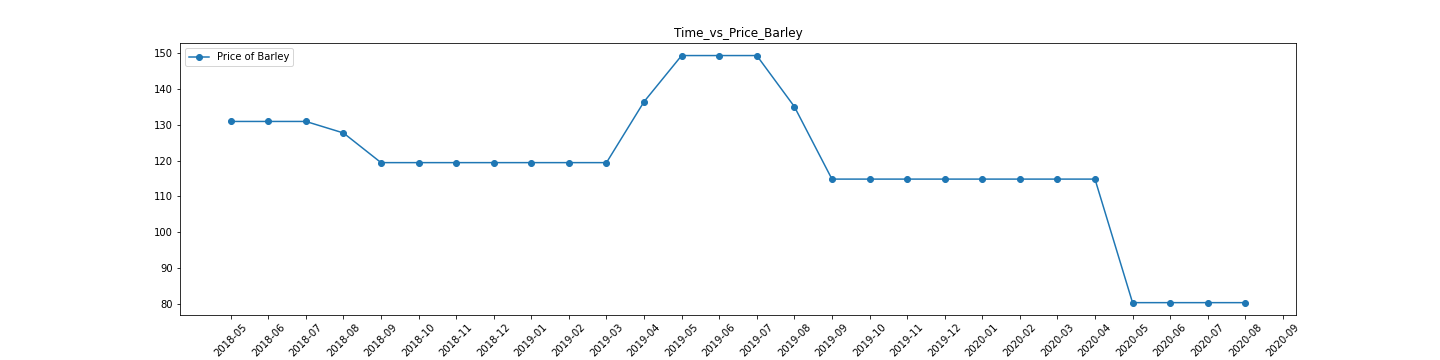
\includegraphics[scale=0.3]{Graphics/Time_vs_Price_Barley.png}
	\end{center}
	\caption{Price of barley in nominal values}
	\label{fig:log-archi}
\end{figure}
\begin{figure} [H]
	\begin{center}
		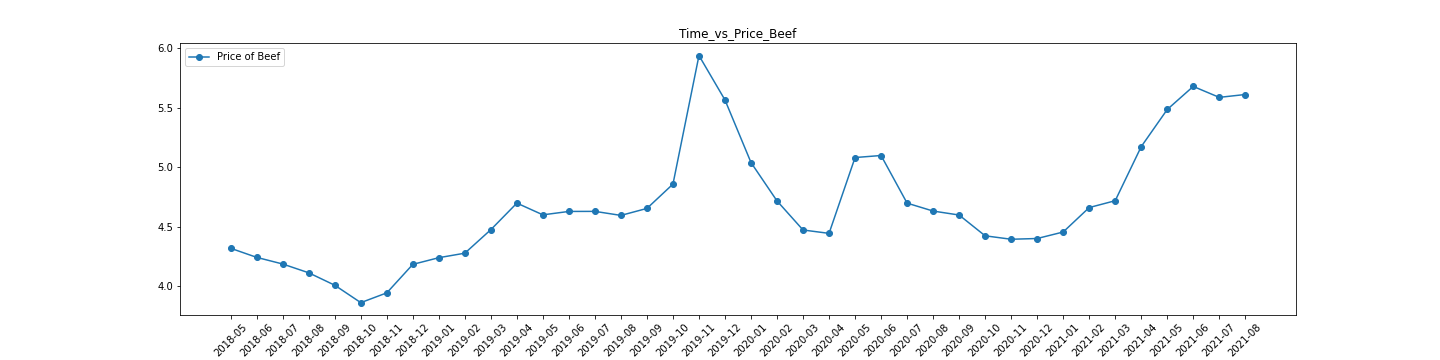
\includegraphics[scale=0.3]{Graphics/Time_vs_Price_Beef.png}
	\end{center}
	\caption{Price of beef in nominal values}
	\label{fig:log-archi}
\end{figure}
\begin{figure} [H]
	\begin{center}
		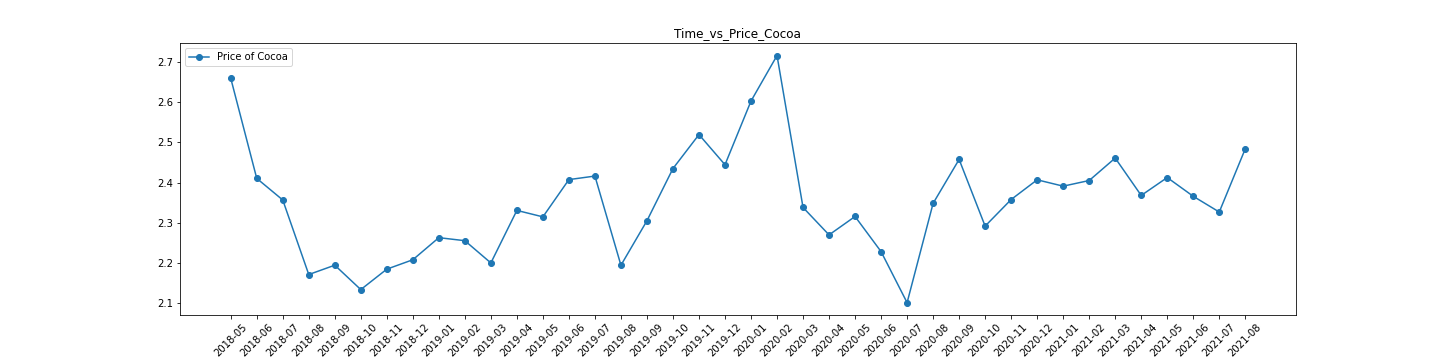
\includegraphics[scale=0.3]{Graphics/Time_vs_Price_Cocoa.png}
	\end{center}
	\caption{Price of cocoa in nominal values}
	\label{fig:log-archi}
\end{figure}
\begin{figure} [H]
	\begin{center}
		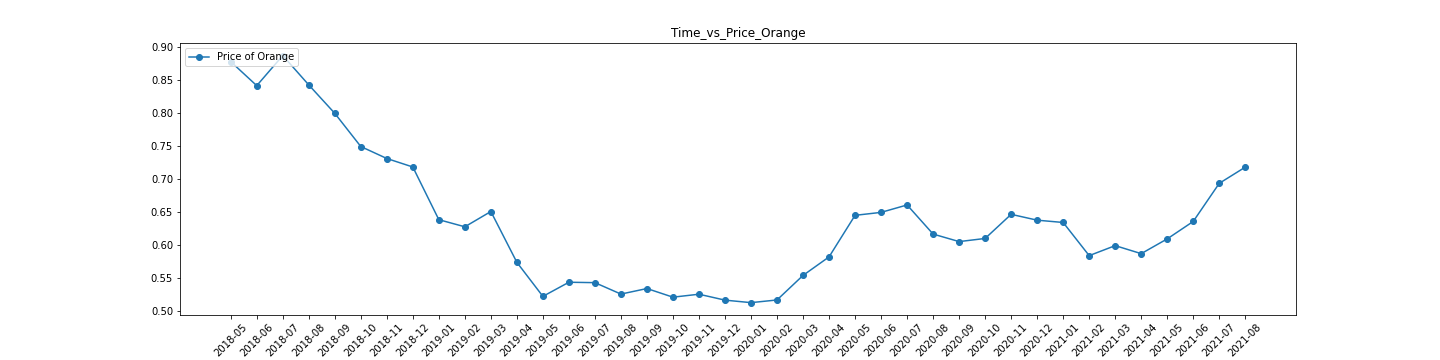
\includegraphics[scale=0.3]{Graphics/Time_vs_Price_Orange.png}
	\end{center}
	\caption{Price of orange in nominal values}
	\label{fig:log-archi}
\end{figure}
\begin{figure} [H]
	\begin{center}
		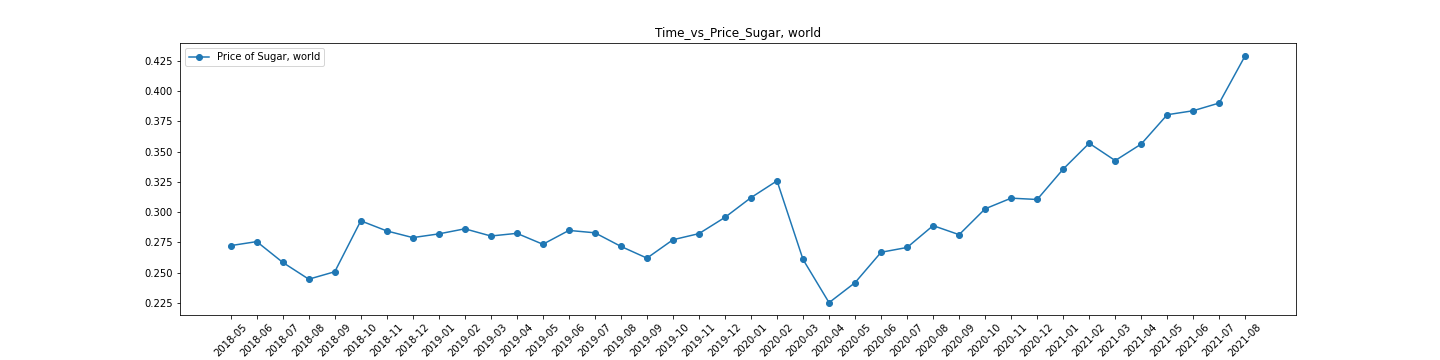
\includegraphics[scale=0.3]{Graphics/Time_vs_Price_Sugar, world.png}
	\end{center}
	\caption{Price of sugar in nominal values}
	\label{fig:log-archi}
\end{figure}
\begin{figure} [H]
	\begin{center}
		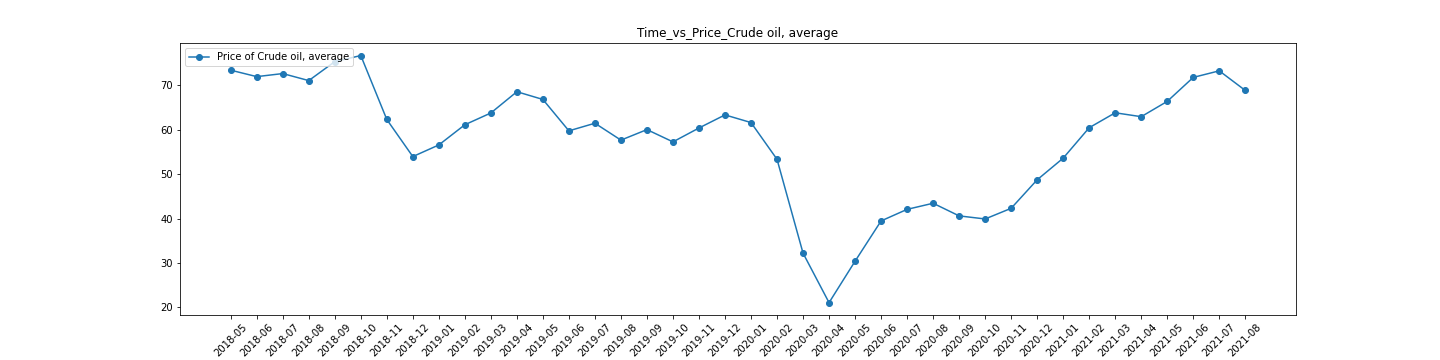
\includegraphics[scale=0.3]{Graphics/Time_vs_Price_Crude oil, average.png}
	\end{center}
	\caption{Price of crude oil in nominal values}
	\label{fig:log-archi}
\end{figure}
\begin{figure} [H]
	\begin{center}
		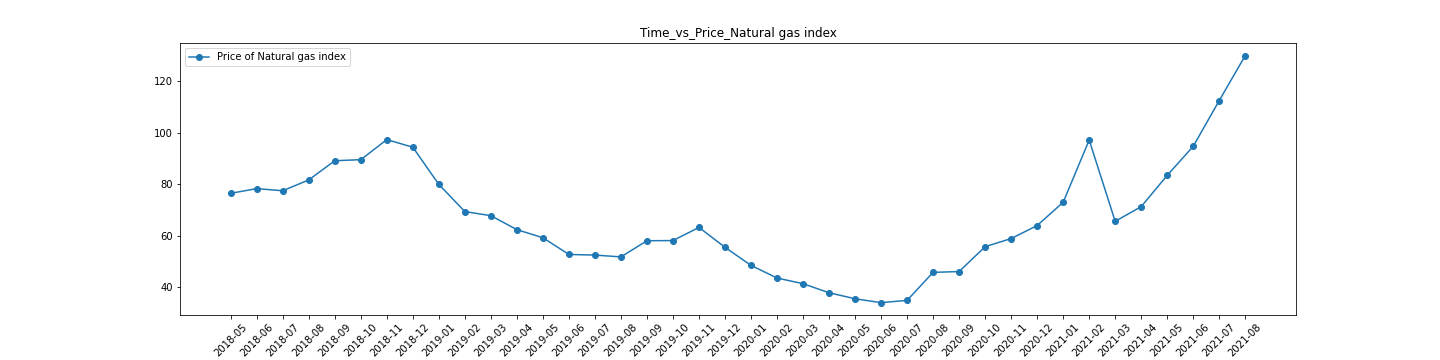
\includegraphics[scale=0.3]{Graphics/Time_vs_Price_Natural gas index.png}
	\end{center}
	\caption{Price of natural gas in nominal values}
	\label{fig:log-archi}
\end{figure}
\begin{figure} [H]
	\begin{center}
		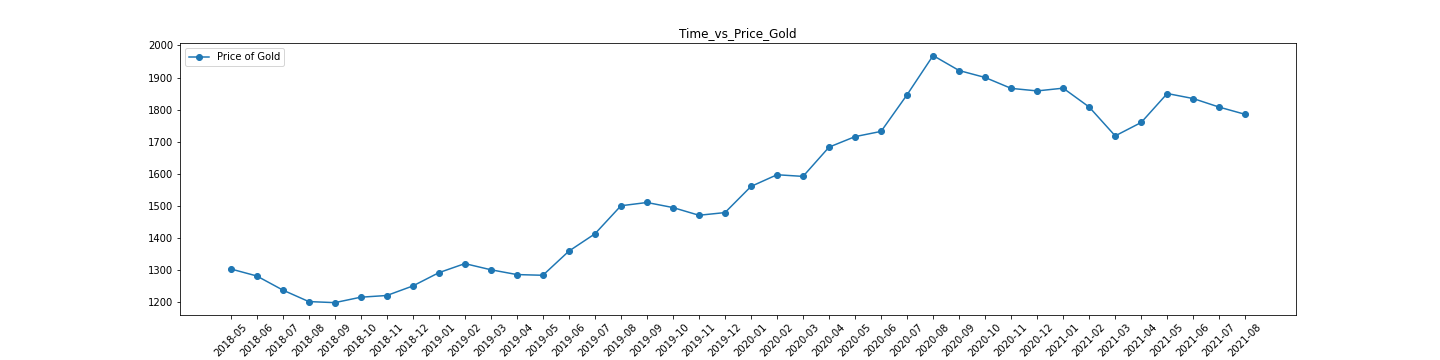
\includegraphics[scale=0.3]{Graphics/Time_vs_Price_Gold.png}
	\end{center}
	\caption{Price of gold in nominal values}
	\label{fig:log-archi}
\end{figure}

\subsection{Figure for G20 inflation with respect to time}
\begin{figure} [H]
	\begin{center}
		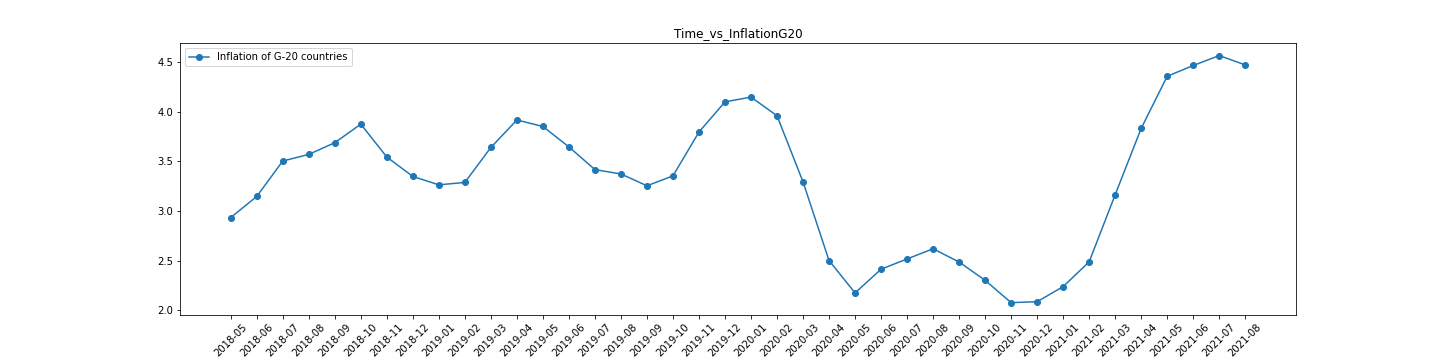
\includegraphics[scale=0.3]{Graphics/Time_vs_InflationG20.png}
	\end{center}
	\caption{G20 Inflation rate }
	\label{fig:log-archi}
\end{figure}


\subsection{Percentage Change Graphs}
In this section we are going to display percentage changes of previously selected commodity prices. then we are going to compare them with global inflation rate.

\begin{figure} [H]
	\begin{center}
		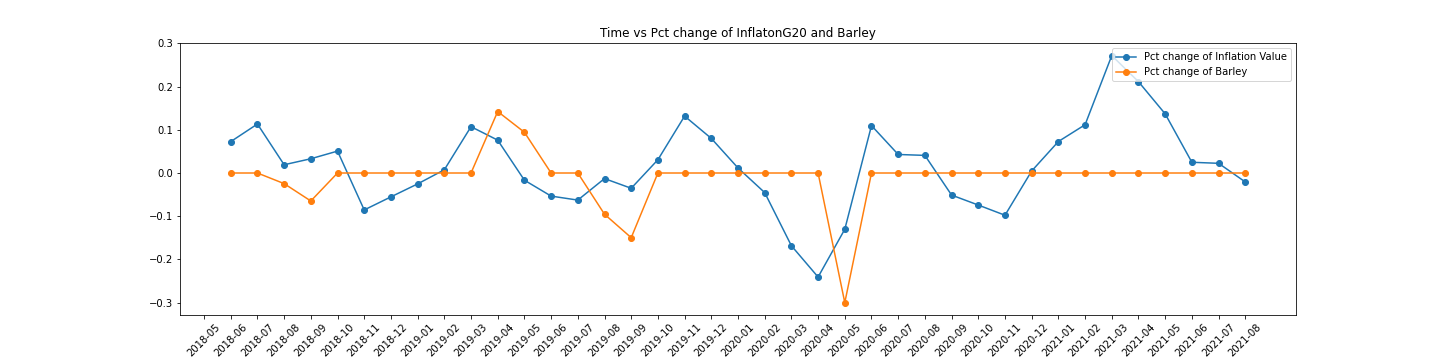
\includegraphics[scale=0.3]{Graphics/pct_change_inflation_and_Barley.png}
	\end{center}
	\caption{Percentage change of barley in comparison to G20 inflation }
	\label{fig:log-archi}
\end{figure}

\begin{figure} [H]
	\begin{center}
		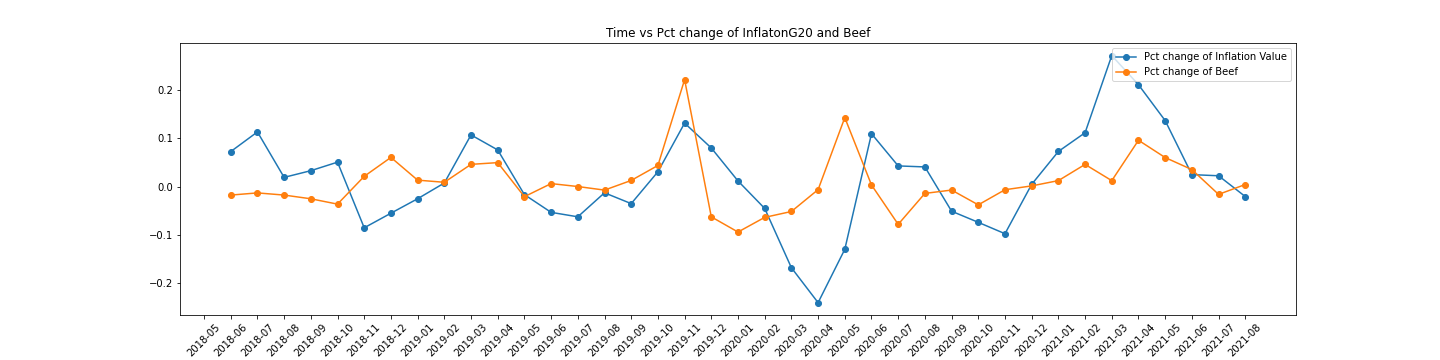
\includegraphics[scale=0.3]{Graphics/pct_change_inflation_and_Beef.png}
	\end{center}
	\caption{Percentage change of beef in comparison to G20 inflation  }
	\label{fig:log-archi}
\end{figure}

\begin{figure} [H]
	\begin{center}
		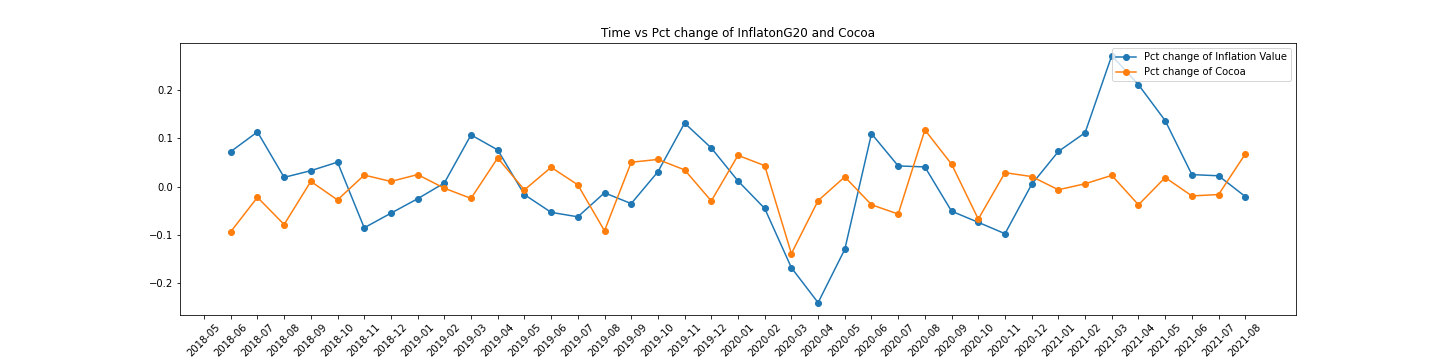
\includegraphics[scale=0.3]{Graphics/pct_change_inflation_and_Cocoa.png}
	\end{center}
	\caption{Percentage change of cocoa in comparison to G20 inflation  }
	\label{fig:log-archi}
\end{figure}


\begin{figure} [H]
	\begin{center}
		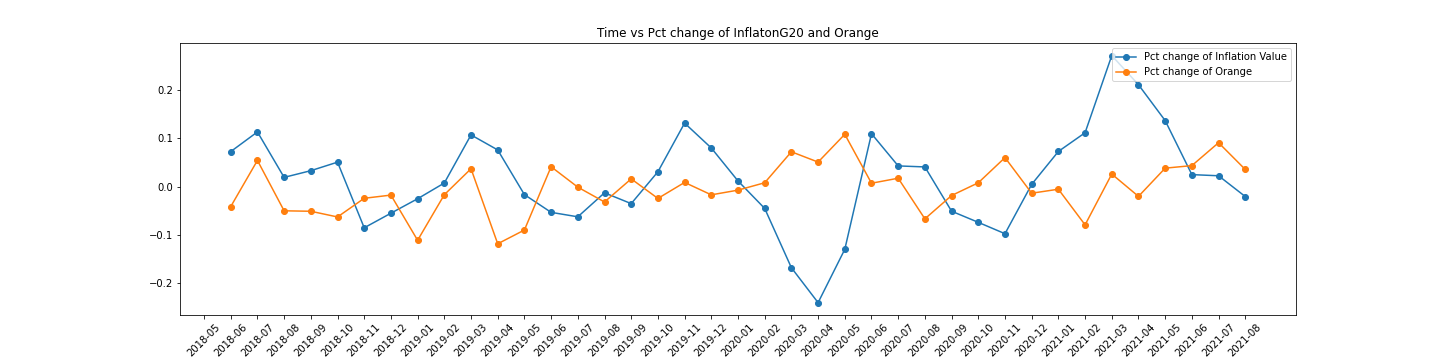
\includegraphics[scale=0.3]{Graphics/pct_change_inflation_and_Orange.png}
	\end{center}
	\caption{Percentage change of orange in comparison to G20 inflation  }
	\label{fig:log-archi}
\end{figure}


\begin{figure} [H]
	\begin{center}
		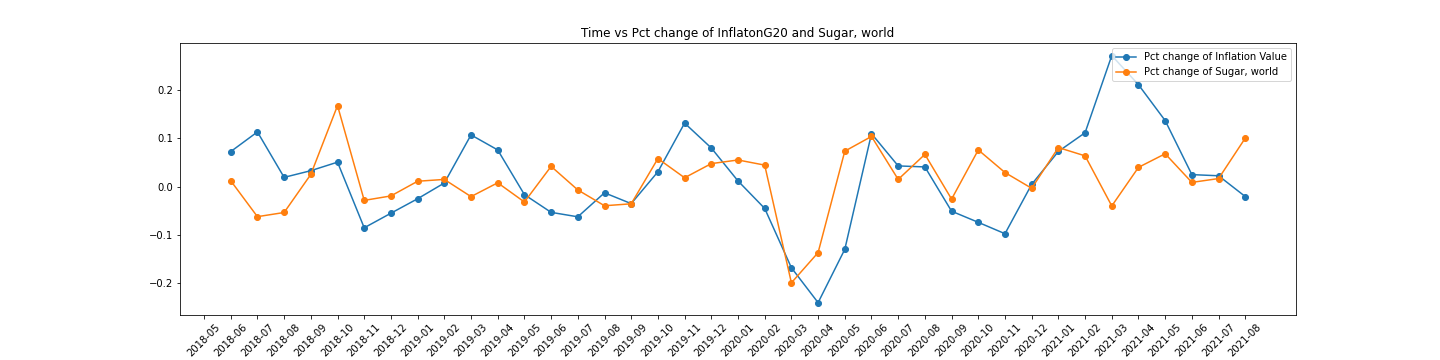
\includegraphics[scale=0.3]{Graphics/pct_change_inflation_and_Sugar, world.png}
	\end{center}
	\caption{Percentage change of sugar in comparison to G20 inflation  }
	\label{fig:log-archi}
\end{figure}


\begin{figure} [H]
	\begin{center}
		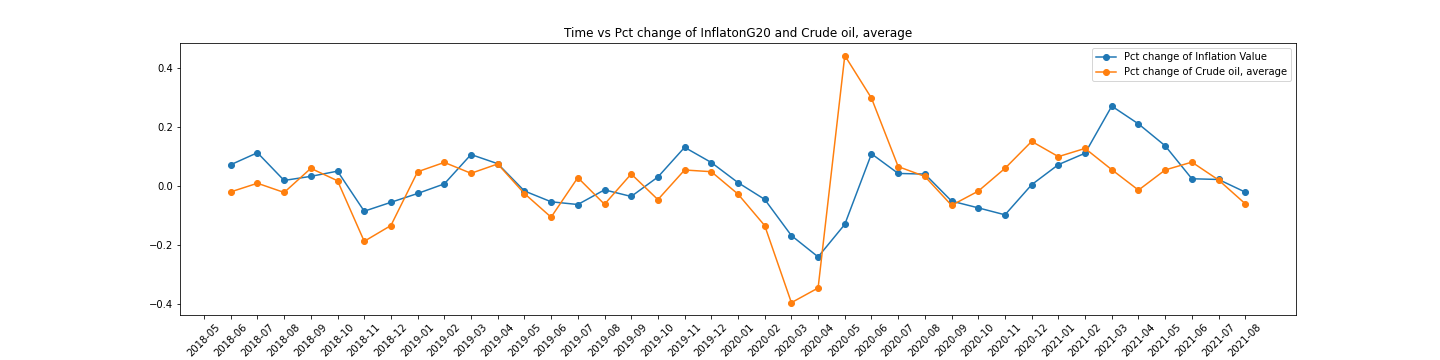
\includegraphics[scale=0.3]{Graphics/pct_change_inflation_and_Crude oil, average.png}
	\end{center}
	\caption{Percentage change of crude oil in comparison to G20 inflation  }
	\label{fig:log-archi}
\end{figure}


\begin{figure} [H]
	\begin{center}
		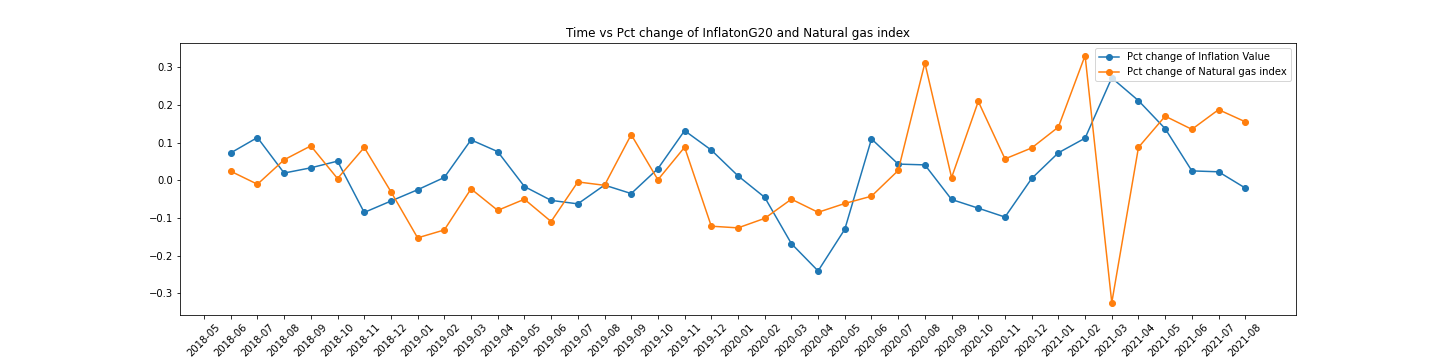
\includegraphics[scale=0.3]{Graphics/pct_change_inflation_and_Natural gas index.png}
	\end{center}
	\caption{Percentage change of natural gas in comparison to G20 inflation  }
	\label{fig:log-archi}
\end{figure}

\begin{figure} [H]
	\begin{center}
		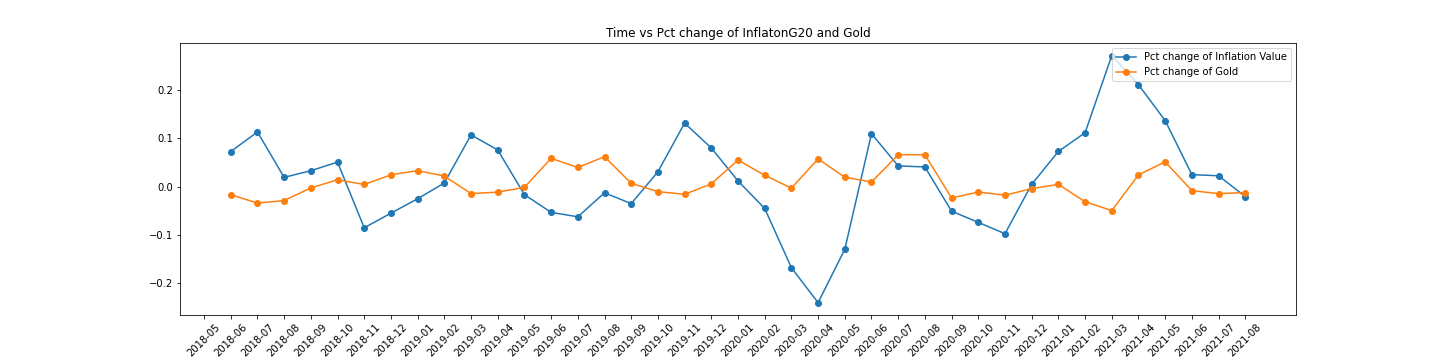
\includegraphics[scale=0.3]{Graphics/pct_change_inflation_and_Gold.png}
	\end{center}
	\caption{Percentage change of gold in comparison to G20 inflation  }
	\label{fig:log-archi}
\end{figure}

\begin{figure} [H]
	\begin{center}
		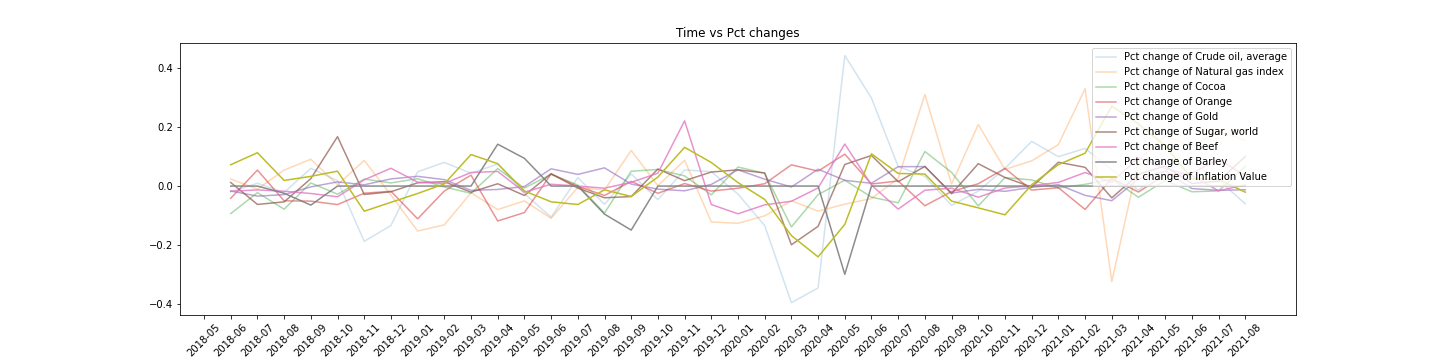
\includegraphics[scale=0.3]{Graphics/pct_changes_together.png}
	\end{center}
	\caption{Percentage change of all commodities in comparison to G20 inflation  }
	\label{fig:log-archi}
\end{figure}


\subsection{Discussion}
From the previous graphs we can see that not all commodity prices increase faster than inflation rate. Clearly there is a strong positive correlation between most of the commodity prices and inflation however, from figure 18 we can see that not all commodity prices increase faster than inflation even if they increase faster inflation for some time period it is not true for all time interval we consider. Another example is that from figure 15, we can clearly see that crude oil price didn't increase faster than inflation until 2020-04. After that point, even though it increased faster than inflation until 2020-06, it decreased rapidly afterwards. So we can't conclude that it increase faster than G20 inflation.

\section{Conclusion}

In summary, from our previous analysis we saw that inflation and commodity prices rise and decline in a positively correlated way. However, not all commodity prices increase faster than inflation and overall since commodity prices increase faster than inflation only at some short time intervals and it is not persistent, we can't conclude our statement "Do commodity prices grow faster than global
inflation?"is true. 

\newpage
\singlespacing



%------ To create Appendix with additional stuff -------%
%\newpage
%\appendix
%\section{Appendix}
%Put data files, CAD drawings, additional sketches, etc.

\end{document}
